\documentclass[11pt,t]{beamer}
\usetheme{Madrid}	
\setbeamertemplate{blocks}[rounded][shadow=false] 
\useinnertheme{circles} %% [circles], [rounded], [rectangles], [default]
\setbeamertemplate{infolines}{}
\setbeamertemplate{navigation symbols}{} 
\setbeamertemplate{footline}[page number]{} 

%%%%%%%%%%%%%%%%%%%%%%%%%%%%%%%%%%%%
%% other packages
\usepackage{natbib}
\newcommand{\newblock}{}
\usepackage{color}

%%%%%%%%%%%%%%%%%%%%%%%%%%%%%%%%%%%%
%% TITLE META DATA
%%%%%%%%%%%%%%%%%%%%%%%%%%%%%%%%%%%%

%\title[Phylogeographic Statistics Performance]{Evaluating the Performance of Phylogeographic Test Statistics using Complex Simulations}
%%\subtitle[Evolution2009]{Evolution 2009}
%\author[Sukumaran, Holder and Brown]{Jeet Sukumaran, Mark. T. Holder and Rafe M. Brown}
%\institute[KU]{
%  Department of Ecology and Evolutionary Biology\\
%  University of Kansas\\
%  Lawrence, KS\\[1ex]
%  \texttt{jeet@ku.edu\\mtholder@ku.edu\\rafe@ku.edu}
%}
%\date[Evolution 2009]{EVOLUTION 2009}
%Presentation at the Joint Annual Meeting of the Society for the Study of Evolution (SSE), the Society of Systematic Biologists (SSB), and the American Society of Naturalists (ASN)


%%%%%%%%%%%%%%%%%%%%%%%%%%%%%%%%%%%%
%% VARIABLES
%%%%%%%%%%%%%%%%%%%%%%%%%%%%%%%%%%%%

\newcommand{\highlighta}[1]{\textcolor{orange}{#1}}
\newcommand{\highlightb}[1]{\textcolor{red}{#1}}

\begin{document}

%%%%%%%%%%%%%%%%%%%%%%%%%%%%%%%%%%%%
%% TITLE PAGE
%%%%%%%%%%%%%%%%%%%%%%%%%%%%%%%%%%%%

%\begin{frame}[plain]
%  \titlepage
%\end{frame}


%%%%%%%%%%%%%%%%%%%%%%%%%%%%%%%%%%%%
%% TOC
%%%%%%%%%%%%%%%%%%%%%%%%%%%%%%%%%%%%

%\section*{Outline} 
%\begin{frame} 
%\tableofcontents 
%\end{frame} 


%%%%%%%%%%%%%%%%%%%%%%%%%%%%%%%%%%%%
%% MAIN PRESENTATION
%%%%%%%%%%%%%%%%%%%%%%%%%%%%%%%%%%%%

% \frametitle{Phylogeographic Analyses and Hypothesis Testing Methods}
% \begin{block}{Definition} 
%A \alert{set} consists of elements. 
%\end{block} 

\begin{frame}
 \frametitle{The Simulation Model}
 	\begin{block}{The Birth-Death Process}	
		\begin{itemize}
			\item Probability of speciation, birth rate = $\lambda$
			\item Probability of extinction, death rate = $\mu$
		\end{itemize}					
	\end{block}
	\begin{block}{The Geographical Template}
		\begin{columns}
			\begin{column}[c]{0.20 \textwidth}
				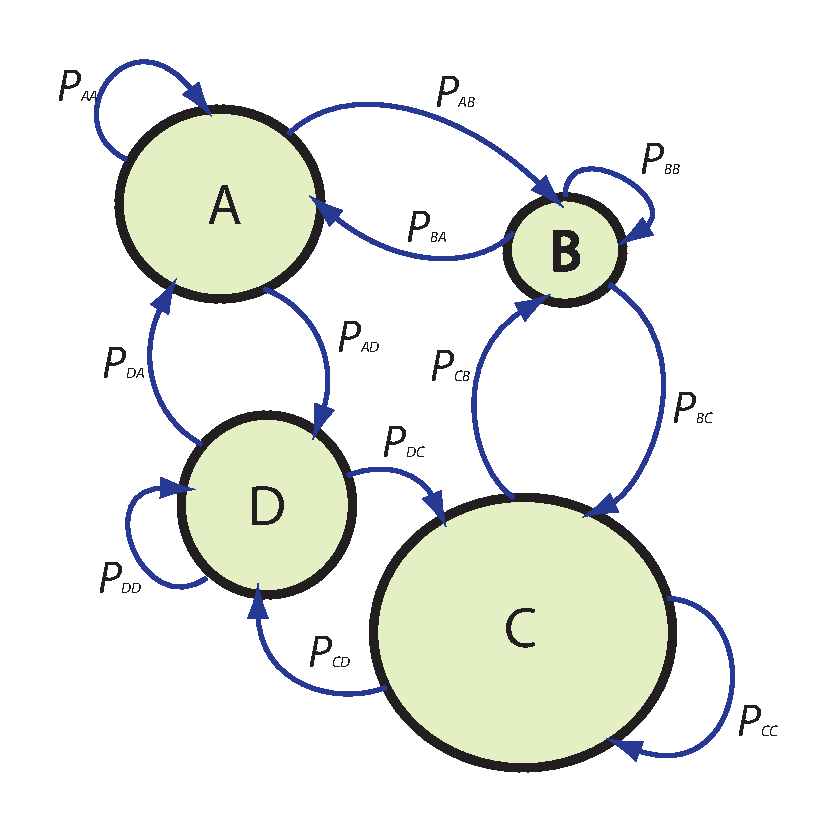
\includegraphics[scale=0.3]{generic-geographical-template.pdf}
			\end{column}
			\begin{column}[T]{0.01 \textwidth}
				{\LARGE  ${\Longrightarrow}$ }
			\end{column}
			\begin{column}[c]{0.40 \textwidth}	
			    \begin{tabular}{c|cccc}
			          & A & B & C & D\\
					\hline	             
			        A & $P_{AA}$ & $P_{AB}$ & $P_{AC}$ & $P_{AD}$ \\
			        B & $P_{BA}$ & $P_{BB}$ & $P_{BC}$ & $P_{BD}$ \\
			        C & $P_{CA}$ & $P_{CB}$ & $P_{CC}$ & $P_{CD}$ \\
			        D & $P_{DA}$ & $P_{DB}$ & $P_{DC}$ & $P_{DD}$ \\
		        \end{tabular}
			\end{column}	        
		\end{columns}
	\end{block}
\end{frame} 

\begin{frame}
	\frametitle{Speciation Modes}
	\begin{itemize}
		\item Sympatric \\
			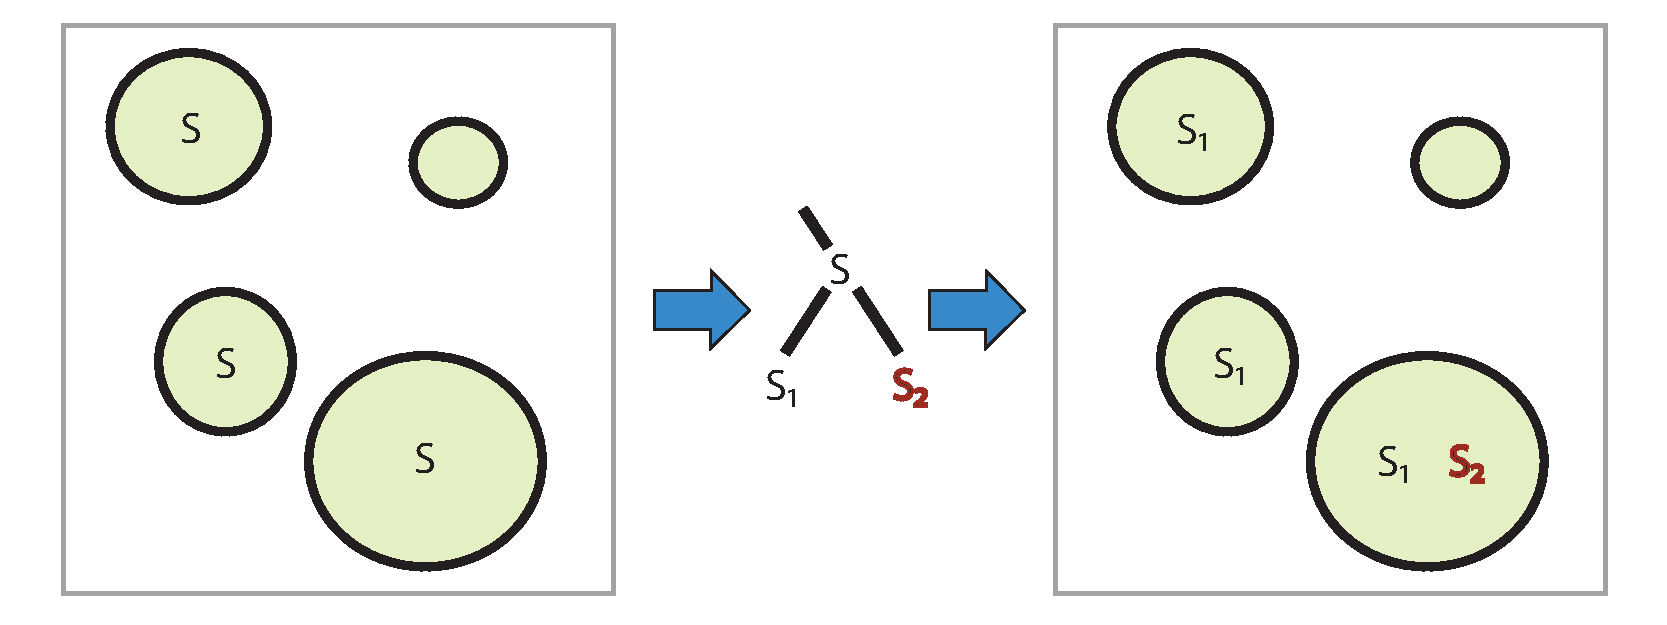
\includegraphics[scale=0.3]{sympatric-speciation.pdf}
		\item Allopatric \\
			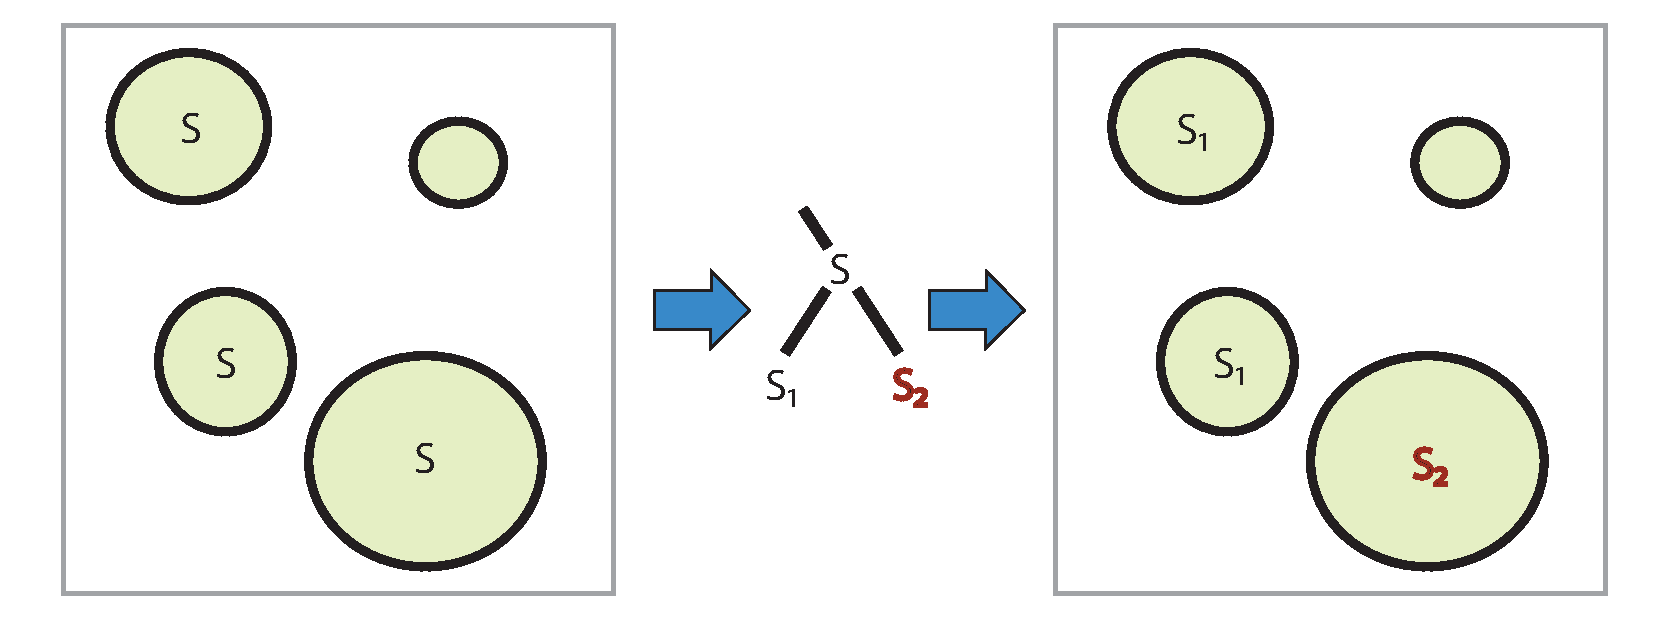
\includegraphics[scale=0.3]{allopatric-speciation.pdf}			
	\end{itemize}
\end{frame}

\begin{frame}
	\frametitle{Simulation Set Up}		
		\begin{itemize}
			\item Set model parameters:
				\begin{itemize}
					\item Birth (speciation) rate, $\lambda$.
					\item Death (extinction) rate, $\mu$.
					\item Geographic template.
					\item Speciation mode.
				\end{itemize}				
		   \item Set termination condition:
				\begin{itemize}
					\item Target diversity: run until total number of species = $T$.
					\item Number of generations: run until number of generations = $G$.
				\end{itemize}						
			\item Specify random number seed.							
		\end{itemize}									
\end{frame}


\begin{frame}
	\frametitle{Simulation Procedure}
	\begin{enumerate}
		\item Initialize: introduce single lineage into a region.
		\item Repeat until $T$ species or $G$ generations, or all species extinct:
			\begin{itemize}
				\item Migration:			
				\begin{itemize} 
					\item For each species in each region, select a destination region for dispersal (including current region, i.e., no dispersal) according to dispersal probability.
					\item Add species to destination region if not already present.
				\end{itemize}
			
				\item Diversification:
				\begin{itemize}	 
					\item For each species in the system, draw a uniform random number, $u \sim U(0,1)$.					
					\item If $u < \lambda$: split lineage.
					\item If $u > \lambda$ and $u < (\lambda + \mu)$: remove lineage.
				\end{itemize}	
			\end{itemize}
		\item Report results.					
	\end{enumerate}
\end{frame}

\begin{frame}
	\frametitle{Simulation Output}
	\begin{itemize}
		\item Incidence (presence/absence) matrix:\\
			\begin{center}
			{\tiny
			    \begin{tabular}{c|cccc}
			          & A & B & C & D\\
					\hline	             
			        $S_{1}$ & 0 & 0 & 1 & 1 \\
			        $S_{2}$ & 1 & 0 & 0 & 1 \\
			        $S_{3}$ & 0 & 1 & 1 & 0 \\
			        .    & . & . & . & . \\
			        .    & . & . & . & . \\
			        .    & . & . & . & . \\			        
			        $S_{T}$ & 1 & 0 & 1 & 1 \\
		        \end{tabular}		
			}
			\end{center}
		\item Phylogeny: \\
			\begin{center}
				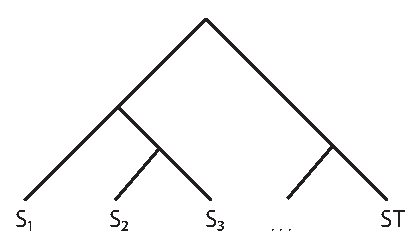
\includegraphics[scale=0.4]{sample-phylogeny.pdf}
			\end{center}				
		\item Summary of total number of lineages and total number of endemic lineages in each region.
		\item Classification tree of areas based on shared species.
	\end{itemize}
\end{frame}

\begin{frame}
	\frametitle{Is This Model Biologically Realistic?}
	\begin{center}
		{\huge NO!}
	\end{center}
\end{frame}

\begin{frame}
	\frametitle{Is This Model Useful?}
	\begin{center}
		{\huge YES!}
	\end{center}
	\begin{itemize}
		\item As a null model, to assess various beta diversity and community diversity studies and statistics that do \textbf{not} take into account evolutionary history.
		\item As a null model, to assess various macro-evolutionary diversification studies and statistics that do \textbf{not} take into account spatial relationships.
		\item To determine whether observed patterns of distributions of island diversity are random with respect to ecological relationships, competition, etc.: if the observed patterns can be replicated under this model, which does not take into account these factors, then we can conclude that simple (random) speciation and (random) dispersal are sufficient explanations for the generation of the observed biotic patterns.
	\end{itemize}
\end{frame}

\begin{frame}
	\frametitle{Application: Geography and the Mid-Domain Effect}
	
	\begin{itemize}
		\item The Mid-Domain Effect as an explanation for the latitudinal gradient in species diversity has been analyzed in terms of "packing" overlapping species ranges into a finite bounded space.
		\item Here, I analyze it as a random effect of cycles of dispersal and diversification under different geographical configurations:	
	\end{itemize}
	
		\begin{columns}		
			\begin{column}[c]{0.4 \textwidth}
				\begin{center}
				``Box'' \\
				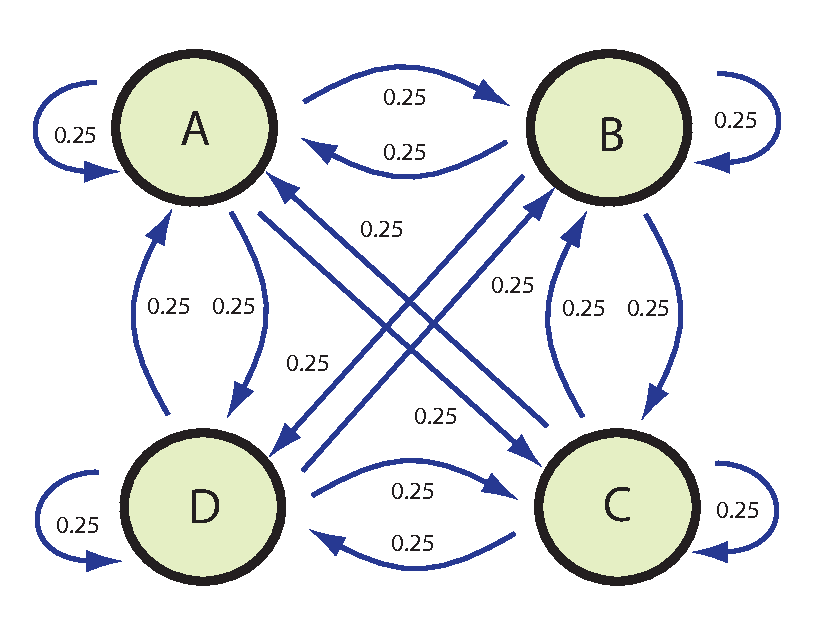
\includegraphics[scale=0.25]{box-model.pdf}
				\end{center}
			\end{column}
			
			\begin{column}[c]{0.4 \textwidth}
				\begin{center}
				``Linear''			\\
				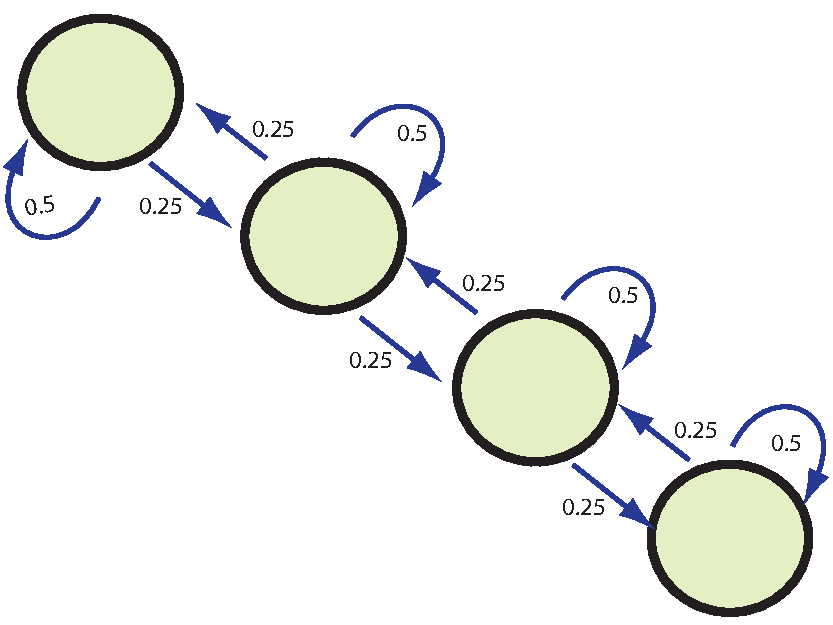
\includegraphics[scale=0.25]{linear-model.pdf}
				\end{center}				
			\end{column}							
		\end{columns}

	\begin{itemize}
	\item Each geographical configuration was run under two birth-death processes: 

	\end{itemize}

\end{frame}


\end{document}






